%%%%%%%%%%%%%%%%%%%%%%%%%%%%%%%%%%%%%%%%%%%%%%%%%%%%%%%%%%%%%%%%%%%%%%%%%%%%%%%%
% WeBWorK Online Homework Delivery System
% Copyright � 2000-2007 The WeBWorK Project, http://openwebwork.sf.net/
% $CVSHeader: webwork2/conf/snippets/hardcopyPreamble.tex,v 1.3 2005/09/17 20:12:01 gage Exp $
% 
% This program is free software; you can redistribute it and/or modify it under
% the terms of either: (a) the GNU General Public License as published by the
% Free Software Foundation; either version 2, or (at your option) any later
% version, or (b) the "Artistic License" which comes with this package.
% 
% This program is distributed in the hope that it will be useful, but WITHOUT
% ANY WARRANTY; without even the implied warranty of MERCHANTABILITY or FITNESS
% FOR A PARTICULAR PURPOSE.  See either the GNU General Public License or the
% Artistic License for more details.
%%%%%%%%%%%%%%%%%%%%%%%%%%%%%%%%%%%%%%%%%%%%%%%%%%%%%%%%%%%%%%%%%%%%%%%%%%%%%%%%

\batchmode
\documentclass[10pt,dvips]{amsart}
\usepackage{amsmath,amsfonts,amssymb,multicol}
\usepackage[pdftex]{graphicx}
\usepackage{epstopdf}  % allows use of eps files with pdftex
\usepackage{epsf}
\usepackage{epsfig}
\usepackage{pslatex}
\usepackage[utf8]{inputenc}
\pagestyle{plain}
\textheight 9in
\oddsidemargin = -0.42in
\evensidemargin = -0.42in
\textwidth= 7.28in
\columnsep = .25in
\columnseprule = .4pt
\def\endline{\bigskip\hrule width \hsize height 0.8pt }
\newcommand{\lt}{<}
\newcommand{\gt}{>}
\newcommand{\less}{<}
\newcommand{\grt}{>}

% BEGIN capa tex macros

\newcommand{\capa}{{\sl C\kern-.10em\raise-.00ex\hbox{\rm A}\kern-.22em%
{\sl P}\kern-.14em\kern-.01em{\rm A}}}
  
\newenvironment{choicelist}
{\begin{list}{}
	{\setlength{\rightmargin}{0in}\setlength{\leftmargin}{0.13in}
	\setlength{\topsep}{0.05in}\setlength{\itemsep}{0.022in}
	\setlength{\parsep}{0in}\setlength{\belowdisplayskip}{0.04in}
	\setlength{\abovedisplayskip}{0.05in}
	\setlength{\abovedisplayshortskip}{-0.04in}
	\setlength{\belowdisplayshortskip}{0.04in}}
	}
{\end{list}}

% END capa tex macros 

\begin{document}
\voffset=-0.8in
\newpage
\setcounter{page}{1}
\begin{multicols}{2}
\columnwidth=\linewidth
 \end{multicols}

\noindent {\large \bf  }
\hfill
{\large \bf {UCSD\_CSE103}}
% Uncomment the line below if this course has sections. Note that this is a comment in TeX mode since this is only processed by LaTeX
%   {\large \bf { Section:  } }
\par
\noindent{\large \bf {Assignment Final1  due 12/17/2013 at 11:45am PST}}
\par\noindent \bigskip
% Uncomment and edit the line below if this course has a web page. Note that this is a comment in TeX mode.
%See the course web page for information http://yoururl/yourcourse



 \begin{multicols}{2}
\columnwidth=\linewidth
%%%%%%%%%%%%%%%%%%%%%%%%%%%%%%%%%%%%%%%%%%%%%%%%%%%%%%%%%%%%%%%%%%%%%%%%%%%%%%%%
% WeBWorK Online Homework Delivery System
% Copyright � 2000-2007 The WeBWorK Project, http://openwebwork.sf.net/
% $CVSHeader: webwork2/conf/snippets/hardcopyProblemDivider.tex,v 1.3 2004/06/24 21:10:50 dpvc Exp $
% 
% This program is free software; you can redistribute it and/or modify it under
% the terms of either: (a) the GNU General Public License as published by the
% Free Software Foundation; either version 2, or (at your option) any later
% version, or (b) the "Artistic License" which comes with this package.
% 
% This program is distributed in the hope that it will be useful, but WITHOUT
% ANY WARRANTY; without even the implied warranty of MERCHANTABILITY or FITNESS
% FOR A PARTICULAR PURPOSE.  See either the GNU General Public License or the
% Artistic License for more details.
%%%%%%%%%%%%%%%%%%%%%%%%%%%%%%%%%%%%%%%%%%%%%%%%%%%%%%%%%%%%%%%%%%%%%%%%%%%%%%%%

\medskip
\goodbreak
\hrule
\nobreak
\smallskip

      \ifx\pgmlMarker\undefined
        \newdimen\pgmlMarker \pgmlMarker=0.00314159pt  % hack to lett if \newline was used
      \fi
      \ifx\oldnewline\undefined \let\oldnewline=\newline \fi
      \def\newline{\oldnewline\hskip-\pgmlMarker\hskip\pgmlMarker\relax}%
      \parindent=0pt
      \catcode`\^^M=\active
      \def^^M{\ifmmode\else\fi\ignorespaces}%  skip paragraph breaks in the preamble
      \def\par{\ifmmode\else\endgraf\fi\ignorespaces}%
    {\bf 1.} (10 pts) \ifdim\lastskip=\pgmlMarker
  \let\pgmlPar=\relax
 \else
  \let\pgmlPar=\par
  \vadjust{\kern3pt}%
\fi

%%%%%%%%%%%%%%%%%%%%%%%%%%%%%%%%%%%%%%
%
%    definitions for PGML
%

\ifx\pgmlCount\undefined  % don not redefine if multiple files load PGML.pl
  \newcount\pgmlCount
  \newdimen\pgmlPercent
  \newdimen\pgmlPixels  \pgmlPixels=.5pt
\fi
\pgmlPercent=.01\hsize

\def\pgmlSetup{%
  \parskip=0pt \parindent=0pt
%  \ifdim\lastskip=\pgmlMarker\else\par\fi
  \pgmlPar
}%

\def\pgmlIndent{\par\advance\leftskip by 2em \advance\pgmlPercent by .02em \pgmlCount=0}%
\def\pgmlbulletItem{\par\indent\llap{$\bullet$ }\ignorespaces}%
\def\pgmlcircleItem{\par\indent\llap{$\circ$ }\ignorespaces}%
\def\pgmlsquareItem{\par\indent\llap{\vrule height 1ex width .75ex depth -.25ex\ }\ignorespaces}%
\def\pgmlnumericItem{\par\indent\advance\pgmlCount by 1 \llap{\the\pgmlCount. }\ignorespaces}%
\def\pgmlalphaItem{\par\indent{\advance\pgmlCount by `\a \llap{\char\pgmlCount. }}\advance\pgmlCount by 1\ignorespaces}%
\def\pgmlAlphaItem{\par\indent{\advance\pgmlCount by `\A \llap{\char\pgmlCount. }}\advance\pgmlCount by 1\ignorespaces}%
\def\pgmlromanItem{\par\indent\advance\pgmlCount by 1 \llap{\romannumeral\pgmlCount. }\ignorespaces}%
\def\pgmlRomanItem{\par\indent\advance\pgmlCount by 1 \llap{\uppercase\expandafter{\romannumeral\pgmlCount}. }\ignorespaces}%

\def\pgmlCenter{%
  \par \parfillskip=0pt
  \advance\leftskip by 0pt plus .5\hsize
  \advance\rightskip by 0pt plus .5\hsize
  \def\pgmlBreak{\break}%
}%
\def\pgmlRight{%
  \par \parfillskip=0pt
  \advance\leftskip by 0pt plus \hsize
  \def\pgmlBreak{\break}%
}%

\def\pgmlBreak{\\}%

\def\pgmlHeading#1{%
  \par\bfseries
  \ifcase#1 \or\huge \or\LARGE \or\large \or\normalsize \or\footnotesize \or\scriptsize \fi
}%

\def\pgmlRule#1#2{%
  \par\noindent
  \hbox{%
    \strut%
    \dimen1=\ht\strutbox%
    \advance\dimen1 by -#2%
    \divide\dimen1 by 2%
    \advance\dimen2 by -\dp\strutbox%
    \raise\dimen1\hbox{\vrule width #1 height #2 depth 0pt}%
  }%
  \par
}%

\def\pgmlIC#1{\futurelet\pgmlNext\pgmlCheckIC}%
\def\pgmlCheckIC{\ifx\pgmlNext\pgmlSpace \/\fi}%
{\def\getSpace#1{\global\let\pgmlSpace= }\getSpace{} }%

{\catcode`\ =12\global\let\pgmlSpaceChar= }%
{\obeylines\gdef\pgmlPreformatted{\par\small\ttfamily\hsize=10\hsize\obeyspaces\obeylines\let^^M=\pgmlNL\pgmlNL}}%
\def\pgmlNL{\par\bgroup\catcode`\ =12\pgmlTestSpace}%
\def\pgmlTestSpace{\futurelet\next\pgmlTestChar}%
\def\pgmlTestChar{\ifx\next\pgmlSpaceChar\ \pgmlTestNext\fi\egroup}%
\def\pgmlTestNext\fi\egroup#1{\fi\pgmlTestSpace}%

\def^^M{\ifmmode\else\space\fi\ignorespaces}%
%%%%%%%%%%%%%%%%%%%%%%%%%%%%%%%%%%%%%%
{\pgmlSetup
How many strings of 4 lower case letters are there that contain at least 2 of the letters in the range a-d inclusive?
\vskip\baselineskip
Hint: look at the complement: how many strings contain no letters in a-d, and how many strings contain exactly one letter in a-d?
\vskip\baselineskip
\mbox{\parbox[t]{23ex}{\hrulefill}}
\par}%
%%%%%%%%%%%%%%%%%%%%%%%%%%%%%%%%%%%%%%%%%%%%%%%%%%%%%%%%%%%%%%%%%%%%%%%%%%%%%%%%
% WeBWorK Online Homework Delivery System
% Copyright � 2000-2007 The WeBWorK Project, http://openwebwork.sf.net/
% $CVSHeader: webwork2/conf/snippets/hardcopyProblemDivider.tex,v 1.3 2004/06/24 21:10:50 dpvc Exp $
% 
% This program is free software; you can redistribute it and/or modify it under
% the terms of either: (a) the GNU General Public License as published by the
% Free Software Foundation; either version 2, or (at your option) any later
% version, or (b) the "Artistic License" which comes with this package.
% 
% This program is distributed in the hope that it will be useful, but WITHOUT
% ANY WARRANTY; without even the implied warranty of MERCHANTABILITY or FITNESS
% FOR A PARTICULAR PURPOSE.  See either the GNU General Public License or the
% Artistic License for more details.
%%%%%%%%%%%%%%%%%%%%%%%%%%%%%%%%%%%%%%%%%%%%%%%%%%%%%%%%%%%%%%%%%%%%%%%%%%%%%%%%

\medskip
\goodbreak
\hrule
\nobreak
\smallskip

      \ifx\pgmlMarker\undefined
        \newdimen\pgmlMarker \pgmlMarker=0.00314159pt  % hack to lett if \newline was used
      \fi
      \ifx\oldnewline\undefined \let\oldnewline=\newline \fi
      \def\newline{\oldnewline\hskip-\pgmlMarker\hskip\pgmlMarker\relax}%
      \parindent=0pt
      \catcode`\^^M=\active
      \def^^M{\ifmmode\else\fi\ignorespaces}%  skip paragraph breaks in the preamble
      \def\par{\ifmmode\else\endgraf\fi\ignorespaces}%
    {\bf 2.} (8 pts) \ifdim\lastskip=\pgmlMarker
  \let\pgmlPar=\relax
 \else
  \let\pgmlPar=\par
  \vadjust{\kern3pt}%
\fi

%%%%%%%%%%%%%%%%%%%%%%%%%%%%%%%%%%%%%%
%
%    definitions for PGML
%

\ifx\pgmlCount\undefined  % don not redefine if multiple files load PGML.pl
  \newcount\pgmlCount
  \newdimen\pgmlPercent
  \newdimen\pgmlPixels  \pgmlPixels=.5pt
\fi
\pgmlPercent=.01\hsize

\def\pgmlSetup{%
  \parskip=0pt \parindent=0pt
%  \ifdim\lastskip=\pgmlMarker\else\par\fi
  \pgmlPar
}%

\def\pgmlIndent{\par\advance\leftskip by 2em \advance\pgmlPercent by .02em \pgmlCount=0}%
\def\pgmlbulletItem{\par\indent\llap{$\bullet$ }\ignorespaces}%
\def\pgmlcircleItem{\par\indent\llap{$\circ$ }\ignorespaces}%
\def\pgmlsquareItem{\par\indent\llap{\vrule height 1ex width .75ex depth -.25ex\ }\ignorespaces}%
\def\pgmlnumericItem{\par\indent\advance\pgmlCount by 1 \llap{\the\pgmlCount. }\ignorespaces}%
\def\pgmlalphaItem{\par\indent{\advance\pgmlCount by `\a \llap{\char\pgmlCount. }}\advance\pgmlCount by 1\ignorespaces}%
\def\pgmlAlphaItem{\par\indent{\advance\pgmlCount by `\A \llap{\char\pgmlCount. }}\advance\pgmlCount by 1\ignorespaces}%
\def\pgmlromanItem{\par\indent\advance\pgmlCount by 1 \llap{\romannumeral\pgmlCount. }\ignorespaces}%
\def\pgmlRomanItem{\par\indent\advance\pgmlCount by 1 \llap{\uppercase\expandafter{\romannumeral\pgmlCount}. }\ignorespaces}%

\def\pgmlCenter{%
  \par \parfillskip=0pt
  \advance\leftskip by 0pt plus .5\hsize
  \advance\rightskip by 0pt plus .5\hsize
  \def\pgmlBreak{\break}%
}%
\def\pgmlRight{%
  \par \parfillskip=0pt
  \advance\leftskip by 0pt plus \hsize
  \def\pgmlBreak{\break}%
}%

\def\pgmlBreak{\\}%

\def\pgmlHeading#1{%
  \par\bfseries
  \ifcase#1 \or\huge \or\LARGE \or\large \or\normalsize \or\footnotesize \or\scriptsize \fi
}%

\def\pgmlRule#1#2{%
  \par\noindent
  \hbox{%
    \strut%
    \dimen1=\ht\strutbox%
    \advance\dimen1 by -#2%
    \divide\dimen1 by 2%
    \advance\dimen2 by -\dp\strutbox%
    \raise\dimen1\hbox{\vrule width #1 height #2 depth 0pt}%
  }%
  \par
}%

\def\pgmlIC#1{\futurelet\pgmlNext\pgmlCheckIC}%
\def\pgmlCheckIC{\ifx\pgmlNext\pgmlSpace \/\fi}%
{\def\getSpace#1{\global\let\pgmlSpace= }\getSpace{} }%

{\catcode`\ =12\global\let\pgmlSpaceChar= }%
{\obeylines\gdef\pgmlPreformatted{\par\small\ttfamily\hsize=10\hsize\obeyspaces\obeylines\let^^M=\pgmlNL\pgmlNL}}%
\def\pgmlNL{\par\bgroup\catcode`\ =12\pgmlTestSpace}%
\def\pgmlTestSpace{\futurelet\next\pgmlTestChar}%
\def\pgmlTestChar{\ifx\next\pgmlSpaceChar\ \pgmlTestNext\fi\egroup}%
\def\pgmlTestNext\fi\egroup#1{\fi\pgmlTestSpace}%

\def^^M{\ifmmode\else\space\fi\ignorespaces}%
%%%%%%%%%%%%%%%%%%%%%%%%%%%%%%%%%%%%%%
{\pgmlSetup
Suppose a pedestrian crosses a busy street either on or off the crosswalk.
Suppose that the probability she uses the cross-walk is 90\%. Furthermore, suppose that the probability of getting hit by a car is $10^{-8}$ when using the cross-walk and $10^{-3}$ when not using the cross-walk. 
\vskip\baselineskip
Suppose the pedestrian crossed the street and was hit by a car, what is the
probability that she was using the cross-walk?\mbox{\parbox[t]{6ex}{\hrulefill}}
\vskip\baselineskip
Suppose the pedestrian crossed the street and was not hit by a car, what is the
probability that she was using the cross-walk?\mbox{\parbox[t]{6ex}{\hrulefill}}
\par}%
%%%%%%%%%%%%%%%%%%%%%%%%%%%%%%%%%%%%%%%%%%%%%%%%%%%%%%%%%%%%%%%%%%%%%%%%%%%%%%%%
% WeBWorK Online Homework Delivery System
% Copyright � 2000-2007 The WeBWorK Project, http://openwebwork.sf.net/
% $CVSHeader: webwork2/conf/snippets/hardcopyProblemDivider.tex,v 1.3 2004/06/24 21:10:50 dpvc Exp $
% 
% This program is free software; you can redistribute it and/or modify it under
% the terms of either: (a) the GNU General Public License as published by the
% Free Software Foundation; either version 2, or (at your option) any later
% version, or (b) the "Artistic License" which comes with this package.
% 
% This program is distributed in the hope that it will be useful, but WITHOUT
% ANY WARRANTY; without even the implied warranty of MERCHANTABILITY or FITNESS
% FOR A PARTICULAR PURPOSE.  See either the GNU General Public License or the
% Artistic License for more details.
%%%%%%%%%%%%%%%%%%%%%%%%%%%%%%%%%%%%%%%%%%%%%%%%%%%%%%%%%%%%%%%%%%%%%%%%%%%%%%%%

\medskip
\goodbreak
\hrule
\nobreak
\smallskip

      \ifx\pgmlMarker\undefined
        \newdimen\pgmlMarker \pgmlMarker=0.00314159pt  % hack to lett if \newline was used
      \fi
      \ifx\oldnewline\undefined \let\oldnewline=\newline \fi
      \def\newline{\oldnewline\hskip-\pgmlMarker\hskip\pgmlMarker\relax}%
      \parindent=0pt
      \catcode`\^^M=\active
      \def^^M{\ifmmode\else\fi\ignorespaces}%  skip paragraph breaks in the preamble
      \def\par{\ifmmode\else\endgraf\fi\ignorespaces}%
    {\bf 3.} (7 pts) \ifdim\lastskip=\pgmlMarker
  \let\pgmlPar=\relax
 \else
  \let\pgmlPar=\par
  \vadjust{\kern3pt}%
\fi

%%%%%%%%%%%%%%%%%%%%%%%%%%%%%%%%%%%%%%
%
%    definitions for PGML
%

\ifx\pgmlCount\undefined  % don not redefine if multiple files load PGML.pl
  \newcount\pgmlCount
  \newdimen\pgmlPercent
  \newdimen\pgmlPixels  \pgmlPixels=.5pt
\fi
\pgmlPercent=.01\hsize

\def\pgmlSetup{%
  \parskip=0pt \parindent=0pt
%  \ifdim\lastskip=\pgmlMarker\else\par\fi
  \pgmlPar
}%

\def\pgmlIndent{\par\advance\leftskip by 2em \advance\pgmlPercent by .02em \pgmlCount=0}%
\def\pgmlbulletItem{\par\indent\llap{$\bullet$ }\ignorespaces}%
\def\pgmlcircleItem{\par\indent\llap{$\circ$ }\ignorespaces}%
\def\pgmlsquareItem{\par\indent\llap{\vrule height 1ex width .75ex depth -.25ex\ }\ignorespaces}%
\def\pgmlnumericItem{\par\indent\advance\pgmlCount by 1 \llap{\the\pgmlCount. }\ignorespaces}%
\def\pgmlalphaItem{\par\indent{\advance\pgmlCount by `\a \llap{\char\pgmlCount. }}\advance\pgmlCount by 1\ignorespaces}%
\def\pgmlAlphaItem{\par\indent{\advance\pgmlCount by `\A \llap{\char\pgmlCount. }}\advance\pgmlCount by 1\ignorespaces}%
\def\pgmlromanItem{\par\indent\advance\pgmlCount by 1 \llap{\romannumeral\pgmlCount. }\ignorespaces}%
\def\pgmlRomanItem{\par\indent\advance\pgmlCount by 1 \llap{\uppercase\expandafter{\romannumeral\pgmlCount}. }\ignorespaces}%

\def\pgmlCenter{%
  \par \parfillskip=0pt
  \advance\leftskip by 0pt plus .5\hsize
  \advance\rightskip by 0pt plus .5\hsize
  \def\pgmlBreak{\break}%
}%
\def\pgmlRight{%
  \par \parfillskip=0pt
  \advance\leftskip by 0pt plus \hsize
  \def\pgmlBreak{\break}%
}%

\def\pgmlBreak{\\}%

\def\pgmlHeading#1{%
  \par\bfseries
  \ifcase#1 \or\huge \or\LARGE \or\large \or\normalsize \or\footnotesize \or\scriptsize \fi
}%

\def\pgmlRule#1#2{%
  \par\noindent
  \hbox{%
    \strut%
    \dimen1=\ht\strutbox%
    \advance\dimen1 by -#2%
    \divide\dimen1 by 2%
    \advance\dimen2 by -\dp\strutbox%
    \raise\dimen1\hbox{\vrule width #1 height #2 depth 0pt}%
  }%
  \par
}%

\def\pgmlIC#1{\futurelet\pgmlNext\pgmlCheckIC}%
\def\pgmlCheckIC{\ifx\pgmlNext\pgmlSpace \/\fi}%
{\def\getSpace#1{\global\let\pgmlSpace= }\getSpace{} }%

{\catcode`\ =12\global\let\pgmlSpaceChar= }%
{\obeylines\gdef\pgmlPreformatted{\par\small\ttfamily\hsize=10\hsize\obeyspaces\obeylines\let^^M=\pgmlNL\pgmlNL}}%
\def\pgmlNL{\par\bgroup\catcode`\ =12\pgmlTestSpace}%
\def\pgmlTestSpace{\futurelet\next\pgmlTestChar}%
\def\pgmlTestChar{\ifx\next\pgmlSpaceChar\ \pgmlTestNext\fi\egroup}%
\def\pgmlTestNext\fi\egroup#1{\fi\pgmlTestSpace}%

\def^^M{\ifmmode\else\space\fi\ignorespaces}%
%%%%%%%%%%%%%%%%%%%%%%%%%%%%%%%%%%%%%%
{\pgmlSetup
You are giving candy to 6 kids. The candy consists of 10 Twix and 8 Milky-ways. Each kids gets at least one Twix. How many ways are there to distribute the candy among the kids?
\vskip\baselineskip
\mbox{\parbox[t]{4.5ex}{\hrulefill}}
\par}%
%%%%%%%%%%%%%%%%%%%%%%%%%%%%%%%%%%%%%%%%%%%%%%%%%%%%%%%%%%%%%%%%%%%%%%%%%%%%%%%%
% WeBWorK Online Homework Delivery System
% Copyright � 2000-2007 The WeBWorK Project, http://openwebwork.sf.net/
% $CVSHeader: webwork2/conf/snippets/hardcopyProblemDivider.tex,v 1.3 2004/06/24 21:10:50 dpvc Exp $
% 
% This program is free software; you can redistribute it and/or modify it under
% the terms of either: (a) the GNU General Public License as published by the
% Free Software Foundation; either version 2, or (at your option) any later
% version, or (b) the "Artistic License" which comes with this package.
% 
% This program is distributed in the hope that it will be useful, but WITHOUT
% ANY WARRANTY; without even the implied warranty of MERCHANTABILITY or FITNESS
% FOR A PARTICULAR PURPOSE.  See either the GNU General Public License or the
% Artistic License for more details.
%%%%%%%%%%%%%%%%%%%%%%%%%%%%%%%%%%%%%%%%%%%%%%%%%%%%%%%%%%%%%%%%%%%%%%%%%%%%%%%%

\medskip
\goodbreak
\hrule
\nobreak
\smallskip
{\bf 4.} (15 pts) \ifdim\lastskip=\pgmlMarker
  \let\pgmlPar=\relax
 \else
  \let\pgmlPar=\par
  \vadjust{\kern3pt}%
\fi

%%%%%%%%%%%%%%%%%%%%%%%%%%%%%%%%%%%%%%
%
%    definitions for PGML
%

\ifx\pgmlCount\undefined  % don not redefine if multiple files load PGML.pl
  \newcount\pgmlCount
  \newdimen\pgmlPercent
  \newdimen\pgmlPixels  \pgmlPixels=.5pt
\fi
\pgmlPercent=.01\hsize

\def\pgmlSetup{%
  \parskip=0pt \parindent=0pt
%  \ifdim\lastskip=\pgmlMarker\else\par\fi
  \pgmlPar
}%

\def\pgmlIndent{\par\advance\leftskip by 2em \advance\pgmlPercent by .02em \pgmlCount=0}%
\def\pgmlbulletItem{\par\indent\llap{$\bullet$ }\ignorespaces}%
\def\pgmlcircleItem{\par\indent\llap{$\circ$ }\ignorespaces}%
\def\pgmlsquareItem{\par\indent\llap{\vrule height 1ex width .75ex depth -.25ex\ }\ignorespaces}%
\def\pgmlnumericItem{\par\indent\advance\pgmlCount by 1 \llap{\the\pgmlCount. }\ignorespaces}%
\def\pgmlalphaItem{\par\indent{\advance\pgmlCount by `\a \llap{\char\pgmlCount. }}\advance\pgmlCount by 1\ignorespaces}%
\def\pgmlAlphaItem{\par\indent{\advance\pgmlCount by `\A \llap{\char\pgmlCount. }}\advance\pgmlCount by 1\ignorespaces}%
\def\pgmlromanItem{\par\indent\advance\pgmlCount by 1 \llap{\romannumeral\pgmlCount. }\ignorespaces}%
\def\pgmlRomanItem{\par\indent\advance\pgmlCount by 1 \llap{\uppercase\expandafter{\romannumeral\pgmlCount}. }\ignorespaces}%

\def\pgmlCenter{%
  \par \parfillskip=0pt
  \advance\leftskip by 0pt plus .5\hsize
  \advance\rightskip by 0pt plus .5\hsize
  \def\pgmlBreak{\break}%
}%
\def\pgmlRight{%
  \par \parfillskip=0pt
  \advance\leftskip by 0pt plus \hsize
  \def\pgmlBreak{\break}%
}%

\def\pgmlBreak{\\}%

\def\pgmlHeading#1{%
  \par\bfseries
  \ifcase#1 \or\huge \or\LARGE \or\large \or\normalsize \or\footnotesize \or\scriptsize \fi
}%

\def\pgmlRule#1#2{%
  \par\noindent
  \hbox{%
    \strut%
    \dimen1=\ht\strutbox%
    \advance\dimen1 by -#2%
    \divide\dimen1 by 2%
    \advance\dimen2 by -\dp\strutbox%
    \raise\dimen1\hbox{\vrule width #1 height #2 depth 0pt}%
  }%
  \par
}%

\def\pgmlIC#1{\futurelet\pgmlNext\pgmlCheckIC}%
\def\pgmlCheckIC{\ifx\pgmlNext\pgmlSpace \/\fi}%
{\def\getSpace#1{\global\let\pgmlSpace= }\getSpace{} }%

{\catcode`\ =12\global\let\pgmlSpaceChar= }%
{\obeylines\gdef\pgmlPreformatted{\par\small\ttfamily\hsize=10\hsize\obeyspaces\obeylines\let^^M=\pgmlNL\pgmlNL}}%
\def\pgmlNL{\par\bgroup\catcode`\ =12\pgmlTestSpace}%
\def\pgmlTestSpace{\futurelet\next\pgmlTestChar}%
\def\pgmlTestChar{\ifx\next\pgmlSpaceChar\ \pgmlTestNext\fi\egroup}%
\def\pgmlTestNext\fi\egroup#1{\fi\pgmlTestSpace}%

\def^^M{\ifmmode\else\space\fi\ignorespaces}%
%%%%%%%%%%%%%%%%%%%%%%%%%%%%%%%%%%%%%%
{\pgmlSetup
For the following joint probability matrices, fill in the missing values and answer the questions. 
\par}%

\par\smallskip\begin{center}\begin{tabular}{|c|c|c|c|c|} \hline

 & X=1   &  X=2   & X=3  &Marginal over Y \\ \hline 

Y=1 & 1/10 & & &3/10 \\ \hline 

Y=2 & 1/5  &1/10 &0 &3/10 \\ \hline 

Y=3 &1/5 & 1/5 & 0  & 2/5  \\ \hline 

Marginal over X &   & 2/5  & 1/10  &* \\ \hline 


\end {tabular}\end{center}\par\smallskip


{\pgmlSetup
{\pgmlIndent\let\pgmlItem=\pgmlbulletItem
\pgmlItem{}Are $X$ and $Y$ dependent? \mbox{\parbox[t]{5ex}{\hrulefill}}

\pgmlItem{}Are $X$ and $Y$ correlated? \mbox{\parbox[t]{5ex}{\hrulefill}}

\par}%
\par}%
{\pgmlSetup
{\pgmlIndent\let\pgmlItem=\pgmlbulletItem
\pgmlItem{}$P(Y=3|X=2) = $ \mbox{\parbox[t]{5ex}{\hrulefill}}
\pgmlRule{100\pgmlPercent}{1\pgmlPixels}%

\par}%
\par}%

\par\smallskip\begin{center}\begin{tabular}{|c|c|c|c|c|} \hline

 & X=1   &  X=2   & X=3  &Marginal over Y \\ \hline 

Y=1 & 1/15 &1/15 &1/15 & \\ \hline 

Y=2 & 2/15  &2/15 &2/15 &2/5 \\ \hline 

Y=3 & & 2/15 &   & 2/5  \\ \hline 

Marginal over X & 1/3  & 1/3  & 1/3  &* \\ \hline 


\end {tabular}\end{center}\par\smallskip


{\pgmlSetup
{\pgmlIndent\let\pgmlItem=\pgmlbulletItem
\pgmlItem{}Are $X$ and $Y$ dependent? \mbox{\parbox[t]{5ex}{\hrulefill}}

\pgmlItem{}Are $X$ and $Y$ correlated? \mbox{\parbox[t]{5ex}{\hrulefill}}

\par}%
\par}%
{\pgmlSetup
{\pgmlIndent\let\pgmlItem=\pgmlbulletItem
\pgmlItem{}$P(X=1|Y=2) = $ \mbox{\parbox[t]{5ex}{\hrulefill}}
\pgmlRule{100\pgmlPercent}{1\pgmlPixels}%

\par}%
\par}%

\par\smallskip\begin{center}\begin{tabular}{|c|c|c|c|c|} \hline

 & X=1   &  X=2   & X=3  &Marginal over Y \\ \hline 

Y=1 & 1/8 &0 &1/8 &1/4 \\ \hline 

Y=2 & 0  &1/2 &0 & \\ \hline 

Y=3 &1/8 & 0 & 1/8  & 1/4  \\ \hline 

Marginal over X & 1/4  &   &   &* \\ \hline 


\end {tabular}\end{center}\par\smallskip


{\pgmlSetup
{\pgmlIndent\let\pgmlItem=\pgmlbulletItem
\pgmlItem{}Are $X$ and $Y$ dependent? \mbox{\parbox[t]{5ex}{\hrulefill}}

\pgmlItem{}Are $X$ and $Y$ correlated? \mbox{\parbox[t]{5ex}{\hrulefill}}

\par}%
\par}%
{\pgmlSetup
{\pgmlIndent\let\pgmlItem=\pgmlbulletItem
\pgmlItem{}$P(Y=2|X=2) = $ \mbox{\parbox[t]{5ex}{\hrulefill}}
\pgmlRule{100\pgmlPercent}{1\pgmlPixels}%

\par}%
\par}%
%%%%%%%%%%%%%%%%%%%%%%%%%%%%%%%%%%%%%%%%%%%%%%%%%%%%%%%%%%%%%%%%%%%%%%%%%%%%%%%%
% WeBWorK Online Homework Delivery System
% Copyright � 2000-2007 The WeBWorK Project, http://openwebwork.sf.net/
% $CVSHeader: webwork2/conf/snippets/hardcopyProblemDivider.tex,v 1.3 2004/06/24 21:10:50 dpvc Exp $
% 
% This program is free software; you can redistribute it and/or modify it under
% the terms of either: (a) the GNU General Public License as published by the
% Free Software Foundation; either version 2, or (at your option) any later
% version, or (b) the "Artistic License" which comes with this package.
% 
% This program is distributed in the hope that it will be useful, but WITHOUT
% ANY WARRANTY; without even the implied warranty of MERCHANTABILITY or FITNESS
% FOR A PARTICULAR PURPOSE.  See either the GNU General Public License or the
% Artistic License for more details.
%%%%%%%%%%%%%%%%%%%%%%%%%%%%%%%%%%%%%%%%%%%%%%%%%%%%%%%%%%%%%%%%%%%%%%%%%%%%%%%%

\medskip
\goodbreak
\hrule
\nobreak
\smallskip

      \ifx\pgmlMarker\undefined
        \newdimen\pgmlMarker \pgmlMarker=0.00314159pt  % hack to lett if \newline was used
      \fi
      \ifx\oldnewline\undefined \let\oldnewline=\newline \fi
      \def\newline{\oldnewline\hskip-\pgmlMarker\hskip\pgmlMarker\relax}%
      \parindent=0pt
      \catcode`\^^M=\active
      \def^^M{\ifmmode\else\fi\ignorespaces}%  skip paragraph breaks in the preamble
      \def\par{\ifmmode\else\endgraf\fi\ignorespaces}%
    {\bf 5.} (10 pts) \ifdim\lastskip=\pgmlMarker
  \let\pgmlPar=\relax
 \else
  \let\pgmlPar=\par
  \vadjust{\kern3pt}%
\fi

%%%%%%%%%%%%%%%%%%%%%%%%%%%%%%%%%%%%%%
%
%    definitions for PGML
%

\ifx\pgmlCount\undefined  % don not redefine if multiple files load PGML.pl
  \newcount\pgmlCount
  \newdimen\pgmlPercent
  \newdimen\pgmlPixels  \pgmlPixels=.5pt
\fi
\pgmlPercent=.01\hsize

\def\pgmlSetup{%
  \parskip=0pt \parindent=0pt
%  \ifdim\lastskip=\pgmlMarker\else\par\fi
  \pgmlPar
}%

\def\pgmlIndent{\par\advance\leftskip by 2em \advance\pgmlPercent by .02em \pgmlCount=0}%
\def\pgmlbulletItem{\par\indent\llap{$\bullet$ }\ignorespaces}%
\def\pgmlcircleItem{\par\indent\llap{$\circ$ }\ignorespaces}%
\def\pgmlsquareItem{\par\indent\llap{\vrule height 1ex width .75ex depth -.25ex\ }\ignorespaces}%
\def\pgmlnumericItem{\par\indent\advance\pgmlCount by 1 \llap{\the\pgmlCount. }\ignorespaces}%
\def\pgmlalphaItem{\par\indent{\advance\pgmlCount by `\a \llap{\char\pgmlCount. }}\advance\pgmlCount by 1\ignorespaces}%
\def\pgmlAlphaItem{\par\indent{\advance\pgmlCount by `\A \llap{\char\pgmlCount. }}\advance\pgmlCount by 1\ignorespaces}%
\def\pgmlromanItem{\par\indent\advance\pgmlCount by 1 \llap{\romannumeral\pgmlCount. }\ignorespaces}%
\def\pgmlRomanItem{\par\indent\advance\pgmlCount by 1 \llap{\uppercase\expandafter{\romannumeral\pgmlCount}. }\ignorespaces}%

\def\pgmlCenter{%
  \par \parfillskip=0pt
  \advance\leftskip by 0pt plus .5\hsize
  \advance\rightskip by 0pt plus .5\hsize
  \def\pgmlBreak{\break}%
}%
\def\pgmlRight{%
  \par \parfillskip=0pt
  \advance\leftskip by 0pt plus \hsize
  \def\pgmlBreak{\break}%
}%

\def\pgmlBreak{\\}%

\def\pgmlHeading#1{%
  \par\bfseries
  \ifcase#1 \or\huge \or\LARGE \or\large \or\normalsize \or\footnotesize \or\scriptsize \fi
}%

\def\pgmlRule#1#2{%
  \par\noindent
  \hbox{%
    \strut%
    \dimen1=\ht\strutbox%
    \advance\dimen1 by -#2%
    \divide\dimen1 by 2%
    \advance\dimen2 by -\dp\strutbox%
    \raise\dimen1\hbox{\vrule width #1 height #2 depth 0pt}%
  }%
  \par
}%

\def\pgmlIC#1{\futurelet\pgmlNext\pgmlCheckIC}%
\def\pgmlCheckIC{\ifx\pgmlNext\pgmlSpace \/\fi}%
{\def\getSpace#1{\global\let\pgmlSpace= }\getSpace{} }%

{\catcode`\ =12\global\let\pgmlSpaceChar= }%
{\obeylines\gdef\pgmlPreformatted{\par\small\ttfamily\hsize=10\hsize\obeyspaces\obeylines\let^^M=\pgmlNL\pgmlNL}}%
\def\pgmlNL{\par\bgroup\catcode`\ =12\pgmlTestSpace}%
\def\pgmlTestSpace{\futurelet\next\pgmlTestChar}%
\def\pgmlTestChar{\ifx\next\pgmlSpaceChar\ \pgmlTestNext\fi\egroup}%
\def\pgmlTestNext\fi\egroup#1{\fi\pgmlTestSpace}%

\def^^M{\ifmmode\else\space\fi\ignorespaces}%
%%%%%%%%%%%%%%%%%%%%%%%%%%%%%%%%%%%%%%
{\pgmlSetup
You are given a card deck of 75 cards, consisting all combinations of 15 ranks and 5 suits. Suppose you draw a hand of 5 cards out of this deck, what is the probability that it will be a {\itshape{}straight} ?
\vskip\baselineskip
Recall that a {\itshape{}straight} refers to five cards whose ranks are in sequence, but whose suits are {\bfseries{}not all the same} (otherwise it is called a straight flush). The 1 can be used either as a low card or a high card when forming a straight. For example, both (1,2,3,4,5) and (12,13,14,15,1) are valid straight ranks, but not (13,14,15,1,2).
\vskip\baselineskip
{\pgmlIndent\let\pgmlItem=\pgmlnumericItem
\pgmlItem{}The number of possibilities for the ranks of a straight is \mbox{\parbox[t]{3ex}{\hrulefill}}.
\vskip\baselineskip
\pgmlItem{}The suits can be anything other than all equal, so the number of possibilities for the suits of a straight is \mbox{\parbox[t]{3ex}{\hrulefill}}.
\vskip\baselineskip
\pgmlItem{}Thus the number of straight hands is \mbox{\parbox[t]{3ex}{\hrulefill}}.
\vskip\baselineskip
\pgmlItem{}Finally, the probability that a randomly chosen hand is a straight is \mbox{\parbox[t]{3ex}{\hrulefill}}.

\par}%
\par}%
%%%%%%%%%%%%%%%%%%%%%%%%%%%%%%%%%%%%%%%%%%%%%%%%%%%%%%%%%%%%%%%%%%%%%%%%%%%%%%%%
% WeBWorK Online Homework Delivery System
% Copyright � 2000-2007 The WeBWorK Project, http://openwebwork.sf.net/
% $CVSHeader: webwork2/conf/snippets/hardcopyProblemDivider.tex,v 1.3 2004/06/24 21:10:50 dpvc Exp $
% 
% This program is free software; you can redistribute it and/or modify it under
% the terms of either: (a) the GNU General Public License as published by the
% Free Software Foundation; either version 2, or (at your option) any later
% version, or (b) the "Artistic License" which comes with this package.
% 
% This program is distributed in the hope that it will be useful, but WITHOUT
% ANY WARRANTY; without even the implied warranty of MERCHANTABILITY or FITNESS
% FOR A PARTICULAR PURPOSE.  See either the GNU General Public License or the
% Artistic License for more details.
%%%%%%%%%%%%%%%%%%%%%%%%%%%%%%%%%%%%%%%%%%%%%%%%%%%%%%%%%%%%%%%%%%%%%%%%%%%%%%%%

\medskip
\goodbreak
\hrule
\nobreak
\smallskip
{\bf 6.} (10 pts) \ifdim\lastskip=\pgmlMarker
  \let\pgmlPar=\relax
 \else
  \let\pgmlPar=\par
  \vadjust{\kern3pt}%
\fi

%%%%%%%%%%%%%%%%%%%%%%%%%%%%%%%%%%%%%%
%
%    definitions for PGML
%

\ifx\pgmlCount\undefined  % don not redefine if multiple files load PGML.pl
  \newcount\pgmlCount
  \newdimen\pgmlPercent
  \newdimen\pgmlPixels  \pgmlPixels=.5pt
\fi
\pgmlPercent=.01\hsize

\def\pgmlSetup{%
  \parskip=0pt \parindent=0pt
%  \ifdim\lastskip=\pgmlMarker\else\par\fi
  \pgmlPar
}%

\def\pgmlIndent{\par\advance\leftskip by 2em \advance\pgmlPercent by .02em \pgmlCount=0}%
\def\pgmlbulletItem{\par\indent\llap{$\bullet$ }\ignorespaces}%
\def\pgmlcircleItem{\par\indent\llap{$\circ$ }\ignorespaces}%
\def\pgmlsquareItem{\par\indent\llap{\vrule height 1ex width .75ex depth -.25ex\ }\ignorespaces}%
\def\pgmlnumericItem{\par\indent\advance\pgmlCount by 1 \llap{\the\pgmlCount. }\ignorespaces}%
\def\pgmlalphaItem{\par\indent{\advance\pgmlCount by `\a \llap{\char\pgmlCount. }}\advance\pgmlCount by 1\ignorespaces}%
\def\pgmlAlphaItem{\par\indent{\advance\pgmlCount by `\A \llap{\char\pgmlCount. }}\advance\pgmlCount by 1\ignorespaces}%
\def\pgmlromanItem{\par\indent\advance\pgmlCount by 1 \llap{\romannumeral\pgmlCount. }\ignorespaces}%
\def\pgmlRomanItem{\par\indent\advance\pgmlCount by 1 \llap{\uppercase\expandafter{\romannumeral\pgmlCount}. }\ignorespaces}%

\def\pgmlCenter{%
  \par \parfillskip=0pt
  \advance\leftskip by 0pt plus .5\hsize
  \advance\rightskip by 0pt plus .5\hsize
  \def\pgmlBreak{\break}%
}%
\def\pgmlRight{%
  \par \parfillskip=0pt
  \advance\leftskip by 0pt plus \hsize
  \def\pgmlBreak{\break}%
}%

\def\pgmlBreak{\\}%

\def\pgmlHeading#1{%
  \par\bfseries
  \ifcase#1 \or\huge \or\LARGE \or\large \or\normalsize \or\footnotesize \or\scriptsize \fi
}%

\def\pgmlRule#1#2{%
  \par\noindent
  \hbox{%
    \strut%
    \dimen1=\ht\strutbox%
    \advance\dimen1 by -#2%
    \divide\dimen1 by 2%
    \advance\dimen2 by -\dp\strutbox%
    \raise\dimen1\hbox{\vrule width #1 height #2 depth 0pt}%
  }%
  \par
}%

\def\pgmlIC#1{\futurelet\pgmlNext\pgmlCheckIC}%
\def\pgmlCheckIC{\ifx\pgmlNext\pgmlSpace \/\fi}%
{\def\getSpace#1{\global\let\pgmlSpace= }\getSpace{} }%

{\catcode`\ =12\global\let\pgmlSpaceChar= }%
{\obeylines\gdef\pgmlPreformatted{\par\small\ttfamily\hsize=10\hsize\obeyspaces\obeylines\let^^M=\pgmlNL\pgmlNL}}%
\def\pgmlNL{\par\bgroup\catcode`\ =12\pgmlTestSpace}%
\def\pgmlTestSpace{\futurelet\next\pgmlTestChar}%
\def\pgmlTestChar{\ifx\next\pgmlSpaceChar\ \pgmlTestNext\fi\egroup}%
\def\pgmlTestNext\fi\egroup#1{\fi\pgmlTestSpace}%

\def^^M{\ifmmode\else\space\fi\ignorespaces}%
%%%%%%%%%%%%%%%%%%%%%%%%%%%%%%%%%%%%%%
{\pgmlSetup
You are given a coin that you assume is a fair coin, and you are interested in the probability that the fraction of ``heads'' in the sequence is at least 0.7
\vskip\baselineskip
{\pgmlIndent\let\pgmlItem=\pgmlalphaItem
\pgmlItem{}Suppose the coin is flipped n=100 times 
{\pgmlIndent\let\pgmlItem=\pgmlcircleItem
\pgmlItem{}Write an exact expression for the probability that the number of heads is equal to 0.7$\times$100=70.  \mbox{\parbox[t]{9.5ex}{\hrulefill}}
\pgmlItem{}What Z-score corresponds to getting 70 heads? \mbox{\parbox[t]{8ex}{\hrulefill}}
\pgmlItem{}What is the central limit theorem approximation for the probability that the number of heads is 70 or higher assuming that the coin is fair? \mbox{\parbox[t]{8ex}{\hrulefill}}

\par}%

\pgmlItem{}Suppose that instead of n=100 times we flip the coin n=10000 times.
{\pgmlIndent\let\pgmlItem=\pgmlcircleItem
\pgmlItem{}What Z-score corresponds to getting 0.7$\times$10000=7000 heads? \mbox{\parbox[t]{8ex}{\hrulefill}}
\pgmlItem{}What is the central limit theorem approximation for the probability that the number of heads is 7000 or higher assuming that the coin is fair?\mbox{\parbox[t]{8ex}{\hrulefill}}
\par}%

\par}%
\par}%
{\pgmlSetup
{\pgmlIndent\let\pgmlItem=\pgmlalphaItem
\pgmlItem{}As we increase the number of coin flips $n$, does the probability of the event {\bfseries{}``the number of heads is larger than 0.7$\times n$''} increase,decrease or stay the same? \mbox{\parbox[t]{7ex}{\hrulefill}}
\par}%
\par}%
%%%%%%%%%%%%%%%%%%%%%%%%%%%%%%%%%%%%%%%%%%%%%%%%%%%%%%%%%%%%%%%%%%%%%%%%%%%%%%%%
% WeBWorK Online Homework Delivery System
% Copyright � 2000-2007 The WeBWorK Project, http://openwebwork.sf.net/
% $CVSHeader: webwork2/conf/snippets/hardcopyProblemDivider.tex,v 1.3 2004/06/24 21:10:50 dpvc Exp $
% 
% This program is free software; you can redistribute it and/or modify it under
% the terms of either: (a) the GNU General Public License as published by the
% Free Software Foundation; either version 2, or (at your option) any later
% version, or (b) the "Artistic License" which comes with this package.
% 
% This program is distributed in the hope that it will be useful, but WITHOUT
% ANY WARRANTY; without even the implied warranty of MERCHANTABILITY or FITNESS
% FOR A PARTICULAR PURPOSE.  See either the GNU General Public License or the
% Artistic License for more details.
%%%%%%%%%%%%%%%%%%%%%%%%%%%%%%%%%%%%%%%%%%%%%%%%%%%%%%%%%%%%%%%%%%%%%%%%%%%%%%%%

\medskip
\goodbreak
\hrule
\nobreak
\smallskip
{\bf 7.} (10 pts) \ifdim\lastskip=\pgmlMarker
  \let\pgmlPar=\relax
 \else
  \let\pgmlPar=\par
  \vadjust{\kern3pt}%
\fi

%%%%%%%%%%%%%%%%%%%%%%%%%%%%%%%%%%%%%%
%
%    definitions for PGML
%

\ifx\pgmlCount\undefined  % don not redefine if multiple files load PGML.pl
  \newcount\pgmlCount
  \newdimen\pgmlPercent
  \newdimen\pgmlPixels  \pgmlPixels=.5pt
\fi
\pgmlPercent=.01\hsize

\def\pgmlSetup{%
  \parskip=0pt \parindent=0pt
%  \ifdim\lastskip=\pgmlMarker\else\par\fi
  \pgmlPar
}%

\def\pgmlIndent{\par\advance\leftskip by 2em \advance\pgmlPercent by .02em \pgmlCount=0}%
\def\pgmlbulletItem{\par\indent\llap{$\bullet$ }\ignorespaces}%
\def\pgmlcircleItem{\par\indent\llap{$\circ$ }\ignorespaces}%
\def\pgmlsquareItem{\par\indent\llap{\vrule height 1ex width .75ex depth -.25ex\ }\ignorespaces}%
\def\pgmlnumericItem{\par\indent\advance\pgmlCount by 1 \llap{\the\pgmlCount. }\ignorespaces}%
\def\pgmlalphaItem{\par\indent{\advance\pgmlCount by `\a \llap{\char\pgmlCount. }}\advance\pgmlCount by 1\ignorespaces}%
\def\pgmlAlphaItem{\par\indent{\advance\pgmlCount by `\A \llap{\char\pgmlCount. }}\advance\pgmlCount by 1\ignorespaces}%
\def\pgmlromanItem{\par\indent\advance\pgmlCount by 1 \llap{\romannumeral\pgmlCount. }\ignorespaces}%
\def\pgmlRomanItem{\par\indent\advance\pgmlCount by 1 \llap{\uppercase\expandafter{\romannumeral\pgmlCount}. }\ignorespaces}%

\def\pgmlCenter{%
  \par \parfillskip=0pt
  \advance\leftskip by 0pt plus .5\hsize
  \advance\rightskip by 0pt plus .5\hsize
  \def\pgmlBreak{\break}%
}%
\def\pgmlRight{%
  \par \parfillskip=0pt
  \advance\leftskip by 0pt plus \hsize
  \def\pgmlBreak{\break}%
}%

\def\pgmlBreak{\\}%

\def\pgmlHeading#1{%
  \par\bfseries
  \ifcase#1 \or\huge \or\LARGE \or\large \or\normalsize \or\footnotesize \or\scriptsize \fi
}%

\def\pgmlRule#1#2{%
  \par\noindent
  \hbox{%
    \strut%
    \dimen1=\ht\strutbox%
    \advance\dimen1 by -#2%
    \divide\dimen1 by 2%
    \advance\dimen2 by -\dp\strutbox%
    \raise\dimen1\hbox{\vrule width #1 height #2 depth 0pt}%
  }%
  \par
}%

\def\pgmlIC#1{\futurelet\pgmlNext\pgmlCheckIC}%
\def\pgmlCheckIC{\ifx\pgmlNext\pgmlSpace \/\fi}%
{\def\getSpace#1{\global\let\pgmlSpace= }\getSpace{} }%

{\catcode`\ =12\global\let\pgmlSpaceChar= }%
{\obeylines\gdef\pgmlPreformatted{\par\small\ttfamily\hsize=10\hsize\obeyspaces\obeylines\let^^M=\pgmlNL\pgmlNL}}%
\def\pgmlNL{\par\bgroup\catcode`\ =12\pgmlTestSpace}%
\def\pgmlTestSpace{\futurelet\next\pgmlTestChar}%
\def\pgmlTestChar{\ifx\next\pgmlSpaceChar\ \pgmlTestNext\fi\egroup}%
\def\pgmlTestNext\fi\egroup#1{\fi\pgmlTestSpace}%

\def^^M{\ifmmode\else\space\fi\ignorespaces}%
%%%%%%%%%%%%%%%%%%%%%%%%%%%%%%%%%%%%%%
{\pgmlSetup
Suppose a web-server receives, on average, 60 requests per minute.  Assume that the requests are independent and therefore:
\vskip\baselineskip
{\pgmlIndent\let\pgmlItem=\pgmlnumericItem
\pgmlItem{}The number of requests in any given minute is distributed according to a Poisson distribution and

\pgmlItem{}The time between two consecutive requests is distributed according to an Exponential distribution. 
\par}%
\vskip\baselineskip
{\pgmlIndent\let\pgmlItem=\pgmlcircleItem
\pgmlItem{}What is the probability that it will not receive any request within the first 9 seconds of some particular minute? \mbox{\parbox[t]{8.5ex}{\hrulefill}}
\vskip\baselineskip
\pgmlItem{}What is the probability that it will receive exactly 4 requests during the same period of time? \mbox{\parbox[t]{11ex}{\hrulefill}}
\vskip\baselineskip
\pgmlItem{}What is the probability that the time between the first and the second requests received in a minute would be smaller than 4 seconds?  \mbox{\parbox[t]{7ex}{\hrulefill}}

\par}%
\par}%
%%%%%%%%%%%%%%%%%%%%%%%%%%%%%%%%%%%%%%%%%%%%%%%%%%%%%%%%%%%%%%%%%%%%%%%%%%%%%%%%
% WeBWorK Online Homework Delivery System
% Copyright � 2000-2007 The WeBWorK Project, http://openwebwork.sf.net/
% $CVSHeader: webwork2/conf/snippets/hardcopyProblemDivider.tex,v 1.3 2004/06/24 21:10:50 dpvc Exp $
% 
% This program is free software; you can redistribute it and/or modify it under
% the terms of either: (a) the GNU General Public License as published by the
% Free Software Foundation; either version 2, or (at your option) any later
% version, or (b) the "Artistic License" which comes with this package.
% 
% This program is distributed in the hope that it will be useful, but WITHOUT
% ANY WARRANTY; without even the implied warranty of MERCHANTABILITY or FITNESS
% FOR A PARTICULAR PURPOSE.  See either the GNU General Public License or the
% Artistic License for more details.
%%%%%%%%%%%%%%%%%%%%%%%%%%%%%%%%%%%%%%%%%%%%%%%%%%%%%%%%%%%%%%%%%%%%%%%%%%%%%%%%

\medskip
\goodbreak
\hrule
\nobreak
\smallskip

      \ifx\pgmlMarker\undefined
        \newdimen\pgmlMarker \pgmlMarker=0.00314159pt  % hack to lett if \newline was used
      \fi
      \ifx\oldnewline\undefined \let\oldnewline=\newline \fi
      \def\newline{\oldnewline\hskip-\pgmlMarker\hskip\pgmlMarker\relax}%
      \parindent=0pt
      \catcode`\^^M=\active
      \def^^M{\ifmmode\else\fi\ignorespaces}%  skip paragraph breaks in the preamble
      \def\par{\ifmmode\else\endgraf\fi\ignorespaces}%
    {\bf 8.} (10 pts) \ifdim\lastskip=\pgmlMarker
  \let\pgmlPar=\relax
 \else
  \let\pgmlPar=\par
  \vadjust{\kern3pt}%
\fi

%%%%%%%%%%%%%%%%%%%%%%%%%%%%%%%%%%%%%%
%
%    definitions for PGML
%

\ifx\pgmlCount\undefined  % don not redefine if multiple files load PGML.pl
  \newcount\pgmlCount
  \newdimen\pgmlPercent
  \newdimen\pgmlPixels  \pgmlPixels=.5pt
\fi
\pgmlPercent=.01\hsize

\def\pgmlSetup{%
  \parskip=0pt \parindent=0pt
%  \ifdim\lastskip=\pgmlMarker\else\par\fi
  \pgmlPar
}%

\def\pgmlIndent{\par\advance\leftskip by 2em \advance\pgmlPercent by .02em \pgmlCount=0}%
\def\pgmlbulletItem{\par\indent\llap{$\bullet$ }\ignorespaces}%
\def\pgmlcircleItem{\par\indent\llap{$\circ$ }\ignorespaces}%
\def\pgmlsquareItem{\par\indent\llap{\vrule height 1ex width .75ex depth -.25ex\ }\ignorespaces}%
\def\pgmlnumericItem{\par\indent\advance\pgmlCount by 1 \llap{\the\pgmlCount. }\ignorespaces}%
\def\pgmlalphaItem{\par\indent{\advance\pgmlCount by `\a \llap{\char\pgmlCount. }}\advance\pgmlCount by 1\ignorespaces}%
\def\pgmlAlphaItem{\par\indent{\advance\pgmlCount by `\A \llap{\char\pgmlCount. }}\advance\pgmlCount by 1\ignorespaces}%
\def\pgmlromanItem{\par\indent\advance\pgmlCount by 1 \llap{\romannumeral\pgmlCount. }\ignorespaces}%
\def\pgmlRomanItem{\par\indent\advance\pgmlCount by 1 \llap{\uppercase\expandafter{\romannumeral\pgmlCount}. }\ignorespaces}%

\def\pgmlCenter{%
  \par \parfillskip=0pt
  \advance\leftskip by 0pt plus .5\hsize
  \advance\rightskip by 0pt plus .5\hsize
  \def\pgmlBreak{\break}%
}%
\def\pgmlRight{%
  \par \parfillskip=0pt
  \advance\leftskip by 0pt plus \hsize
  \def\pgmlBreak{\break}%
}%

\def\pgmlBreak{\\}%

\def\pgmlHeading#1{%
  \par\bfseries
  \ifcase#1 \or\huge \or\LARGE \or\large \or\normalsize \or\footnotesize \or\scriptsize \fi
}%

\def\pgmlRule#1#2{%
  \par\noindent
  \hbox{%
    \strut%
    \dimen1=\ht\strutbox%
    \advance\dimen1 by -#2%
    \divide\dimen1 by 2%
    \advance\dimen2 by -\dp\strutbox%
    \raise\dimen1\hbox{\vrule width #1 height #2 depth 0pt}%
  }%
  \par
}%

\def\pgmlIC#1{\futurelet\pgmlNext\pgmlCheckIC}%
\def\pgmlCheckIC{\ifx\pgmlNext\pgmlSpace \/\fi}%
{\def\getSpace#1{\global\let\pgmlSpace= }\getSpace{} }%

{\catcode`\ =12\global\let\pgmlSpaceChar= }%
{\obeylines\gdef\pgmlPreformatted{\par\small\ttfamily\hsize=10\hsize\obeyspaces\obeylines\let^^M=\pgmlNL\pgmlNL}}%
\def\pgmlNL{\par\bgroup\catcode`\ =12\pgmlTestSpace}%
\def\pgmlTestSpace{\futurelet\next\pgmlTestChar}%
\def\pgmlTestChar{\ifx\next\pgmlSpaceChar\ \pgmlTestNext\fi\egroup}%
\def\pgmlTestNext\fi\egroup#1{\fi\pgmlTestSpace}%

\def^^M{\ifmmode\else\space\fi\ignorespaces}%
%%%%%%%%%%%%%%%%%%%%%%%%%%%%%%%%%%%%%%
{\pgmlSetup
Suppose $X_1, ... , X_{86}$ are independent random variables where $X_i \in \{0,1\}$ and $P(X_i = 1) = 0.3$ for $i = 1, ..., n$.
\vskip\baselineskip
Define a random variable $Y = \sum_{i=1}^{86}{(-1)^{i+1} X_i} = X_1 - X_2 + X_3 - X_4 + ... - X_{86}$
\vskip\baselineskip
What is $E[Y]$?  \mbox{\parbox[t]{11ex}{\hrulefill}}
\vskip\baselineskip
What is $Var[Y]$?  \mbox{\parbox[t]{10.5ex}{\hrulefill}}
\vskip\baselineskip
Using Chebyshev's inequality, give un upper bound on $P(|Y| > 30)$?  \mbox{\parbox[t]{14ex}{\hrulefill}}
\par}%
%%%%%%%%%%%%%%%%%%%%%%%%%%%%%%%%%%%%%%%%%%%%%%%%%%%%%%%%%%%%%%%%%%%%%%%%%%%%%%%%
% WeBWorK Online Homework Delivery System
% Copyright � 2000-2007 The WeBWorK Project, http://openwebwork.sf.net/
% $CVSHeader: webwork2/conf/snippets/hardcopyProblemDivider.tex,v 1.3 2004/06/24 21:10:50 dpvc Exp $
% 
% This program is free software; you can redistribute it and/or modify it under
% the terms of either: (a) the GNU General Public License as published by the
% Free Software Foundation; either version 2, or (at your option) any later
% version, or (b) the "Artistic License" which comes with this package.
% 
% This program is distributed in the hope that it will be useful, but WITHOUT
% ANY WARRANTY; without even the implied warranty of MERCHANTABILITY or FITNESS
% FOR A PARTICULAR PURPOSE.  See either the GNU General Public License or the
% Artistic License for more details.
%%%%%%%%%%%%%%%%%%%%%%%%%%%%%%%%%%%%%%%%%%%%%%%%%%%%%%%%%%%%%%%%%%%%%%%%%%%%%%%%

\medskip
\goodbreak
\hrule
\nobreak
\smallskip

      \ifx\pgmlMarker\undefined
        \newdimen\pgmlMarker \pgmlMarker=0.00314159pt  % hack to lett if \newline was used
      \fi
      \ifx\oldnewline\undefined \let\oldnewline=\newline \fi
      \def\newline{\oldnewline\hskip-\pgmlMarker\hskip\pgmlMarker\relax}%
      \parindent=0pt
      \catcode`\^^M=\active
      \def^^M{\ifmmode\else\fi\ignorespaces}%  skip paragraph breaks in the preamble
      \def\par{\ifmmode\else\endgraf\fi\ignorespaces}%
    {\bf 9.} (10 pts) \ifdim\lastskip=\pgmlMarker
  \let\pgmlPar=\relax
 \else
  \let\pgmlPar=\par
  \vadjust{\kern3pt}%
\fi

%%%%%%%%%%%%%%%%%%%%%%%%%%%%%%%%%%%%%%
%
%    definitions for PGML
%

\ifx\pgmlCount\undefined  % don not redefine if multiple files load PGML.pl
  \newcount\pgmlCount
  \newdimen\pgmlPercent
  \newdimen\pgmlPixels  \pgmlPixels=.5pt
\fi
\pgmlPercent=.01\hsize

\def\pgmlSetup{%
  \parskip=0pt \parindent=0pt
%  \ifdim\lastskip=\pgmlMarker\else\par\fi
  \pgmlPar
}%

\def\pgmlIndent{\par\advance\leftskip by 2em \advance\pgmlPercent by .02em \pgmlCount=0}%
\def\pgmlbulletItem{\par\indent\llap{$\bullet$ }\ignorespaces}%
\def\pgmlcircleItem{\par\indent\llap{$\circ$ }\ignorespaces}%
\def\pgmlsquareItem{\par\indent\llap{\vrule height 1ex width .75ex depth -.25ex\ }\ignorespaces}%
\def\pgmlnumericItem{\par\indent\advance\pgmlCount by 1 \llap{\the\pgmlCount. }\ignorespaces}%
\def\pgmlalphaItem{\par\indent{\advance\pgmlCount by `\a \llap{\char\pgmlCount. }}\advance\pgmlCount by 1\ignorespaces}%
\def\pgmlAlphaItem{\par\indent{\advance\pgmlCount by `\A \llap{\char\pgmlCount. }}\advance\pgmlCount by 1\ignorespaces}%
\def\pgmlromanItem{\par\indent\advance\pgmlCount by 1 \llap{\romannumeral\pgmlCount. }\ignorespaces}%
\def\pgmlRomanItem{\par\indent\advance\pgmlCount by 1 \llap{\uppercase\expandafter{\romannumeral\pgmlCount}. }\ignorespaces}%

\def\pgmlCenter{%
  \par \parfillskip=0pt
  \advance\leftskip by 0pt plus .5\hsize
  \advance\rightskip by 0pt plus .5\hsize
  \def\pgmlBreak{\break}%
}%
\def\pgmlRight{%
  \par \parfillskip=0pt
  \advance\leftskip by 0pt plus \hsize
  \def\pgmlBreak{\break}%
}%

\def\pgmlBreak{\\}%

\def\pgmlHeading#1{%
  \par\bfseries
  \ifcase#1 \or\huge \or\LARGE \or\large \or\normalsize \or\footnotesize \or\scriptsize \fi
}%

\def\pgmlRule#1#2{%
  \par\noindent
  \hbox{%
    \strut%
    \dimen1=\ht\strutbox%
    \advance\dimen1 by -#2%
    \divide\dimen1 by 2%
    \advance\dimen2 by -\dp\strutbox%
    \raise\dimen1\hbox{\vrule width #1 height #2 depth 0pt}%
  }%
  \par
}%

\def\pgmlIC#1{\futurelet\pgmlNext\pgmlCheckIC}%
\def\pgmlCheckIC{\ifx\pgmlNext\pgmlSpace \/\fi}%
{\def\getSpace#1{\global\let\pgmlSpace= }\getSpace{} }%

{\catcode`\ =12\global\let\pgmlSpaceChar= }%
{\obeylines\gdef\pgmlPreformatted{\par\small\ttfamily\hsize=10\hsize\obeyspaces\obeylines\let^^M=\pgmlNL\pgmlNL}}%
\def\pgmlNL{\par\bgroup\catcode`\ =12\pgmlTestSpace}%
\def\pgmlTestSpace{\futurelet\next\pgmlTestChar}%
\def\pgmlTestChar{\ifx\next\pgmlSpaceChar\ \pgmlTestNext\fi\egroup}%
\def\pgmlTestNext\fi\egroup#1{\fi\pgmlTestSpace}%

\def^^M{\ifmmode\else\space\fi\ignorespaces}%
%%%%%%%%%%%%%%%%%%%%%%%%%%%%%%%%%%%%%%
{\pgmlSetup
We want to prove that seat-belts save lives. In other words, our goal is to reject the null hypothesis stating that seat-belts do not help.
\vskip\baselineskip
Suppose first that we know that, in general, the probability of a fatality
in a car accident is $q=1\%$.
\vskip\baselineskip
We examine $n=1000$ randomly selected records of accidents where the driver
wore a seat belt. We find that $k=7$ of these accidents were fatal.
\vskip\baselineskip
With what confidence can we conclude that claim is
correct?
\pgmlRule{100\pgmlPercent}{1\pgmlPixels}%
$X_i$ = $i^{th}$ accident was fatal.
\vskip\baselineskip
The null hypothesis is that seat belts make no difference. 
$Pr(X_i=1)=q=0.01$. Alternative hypothesis, $Pr(X_i=1)<q$.
\vskip\baselineskip
The total number of fatal accident under the null hypothesis $S=\sum_i X_i$.
\vskip\baselineskip
$E(S)=$\mbox{\parbox[t]{4.5ex}{\hrulefill}}
\vskip\baselineskip
$var(S)=$\mbox{\parbox[t]{3ex}{\hrulefill}}
$std(S) = $\mbox{\parbox[t]{4ex}{\hrulefill}}
\vskip\baselineskip
$k=7$ is approximately one standard deviation smaller than the mean, in other words, the $z$-score is roughly (write an integer number)\mbox{\parbox[t]{3.5ex}{\hrulefill}}
\vskip\baselineskip
Using this approximation, the {\bfseries{}$p$-value} associated with $k=7$ is \mbox{\parbox[t]{4ex}{\hrulefill}}. 
\par}%
{\pgmlSetup
{\bfseries{}Complete the sentence:} the $p$-value (``is''/''is not'') \mbox{\parbox[t]{4ex}{\hrulefill}} a {\bfseries{}random variable}.
\par}%
%%%%%%%%%%%%%%%%%%%%%%%%%%%%%%%%%%%%%%%%%%%%%%%%%%%%%%%%%%%%%%%%%%%%%%%%%%%%%%%%
% WeBWorK Online Homework Delivery System
% Copyright � 2000-2007 The WeBWorK Project, http://openwebwork.sf.net/
% $CVSHeader: webwork2/conf/snippets/hardcopyProblemDivider.tex,v 1.3 2004/06/24 21:10:50 dpvc Exp $
% 
% This program is free software; you can redistribute it and/or modify it under
% the terms of either: (a) the GNU General Public License as published by the
% Free Software Foundation; either version 2, or (at your option) any later
% version, or (b) the "Artistic License" which comes with this package.
% 
% This program is distributed in the hope that it will be useful, but WITHOUT
% ANY WARRANTY; without even the implied warranty of MERCHANTABILITY or FITNESS
% FOR A PARTICULAR PURPOSE.  See either the GNU General Public License or the
% Artistic License for more details.
%%%%%%%%%%%%%%%%%%%%%%%%%%%%%%%%%%%%%%%%%%%%%%%%%%%%%%%%%%%%%%%%%%%%%%%%%%%%%%%%

\medskip
\goodbreak
\hrule
\nobreak
\smallskip

      \ifx\pgmlMarker\undefined
        \newdimen\pgmlMarker \pgmlMarker=0.00314159pt  % hack to lett if \newline was used
      \fi
      \ifx\oldnewline\undefined \let\oldnewline=\newline \fi
      \def\newline{\oldnewline\hskip-\pgmlMarker\hskip\pgmlMarker\relax}%
      \parindent=0pt
      \catcode`\^^M=\active
      \def^^M{\ifmmode\else\fi\ignorespaces}%  skip paragraph breaks in the preamble
      \def\par{\ifmmode\else\endgraf\fi\ignorespaces}%
    {\bf 10.} (10 pts) \ifdim\lastskip=\pgmlMarker
  \let\pgmlPar=\relax
 \else
  \let\pgmlPar=\par
  \vadjust{\kern3pt}%
\fi

%%%%%%%%%%%%%%%%%%%%%%%%%%%%%%%%%%%%%%
%
%    definitions for PGML
%

\ifx\pgmlCount\undefined  % don not redefine if multiple files load PGML.pl
  \newcount\pgmlCount
  \newdimen\pgmlPercent
  \newdimen\pgmlPixels  \pgmlPixels=.5pt
\fi
\pgmlPercent=.01\hsize

\def\pgmlSetup{%
  \parskip=0pt \parindent=0pt
%  \ifdim\lastskip=\pgmlMarker\else\par\fi
  \pgmlPar
}%

\def\pgmlIndent{\par\advance\leftskip by 2em \advance\pgmlPercent by .02em \pgmlCount=0}%
\def\pgmlbulletItem{\par\indent\llap{$\bullet$ }\ignorespaces}%
\def\pgmlcircleItem{\par\indent\llap{$\circ$ }\ignorespaces}%
\def\pgmlsquareItem{\par\indent\llap{\vrule height 1ex width .75ex depth -.25ex\ }\ignorespaces}%
\def\pgmlnumericItem{\par\indent\advance\pgmlCount by 1 \llap{\the\pgmlCount. }\ignorespaces}%
\def\pgmlalphaItem{\par\indent{\advance\pgmlCount by `\a \llap{\char\pgmlCount. }}\advance\pgmlCount by 1\ignorespaces}%
\def\pgmlAlphaItem{\par\indent{\advance\pgmlCount by `\A \llap{\char\pgmlCount. }}\advance\pgmlCount by 1\ignorespaces}%
\def\pgmlromanItem{\par\indent\advance\pgmlCount by 1 \llap{\romannumeral\pgmlCount. }\ignorespaces}%
\def\pgmlRomanItem{\par\indent\advance\pgmlCount by 1 \llap{\uppercase\expandafter{\romannumeral\pgmlCount}. }\ignorespaces}%

\def\pgmlCenter{%
  \par \parfillskip=0pt
  \advance\leftskip by 0pt plus .5\hsize
  \advance\rightskip by 0pt plus .5\hsize
  \def\pgmlBreak{\break}%
}%
\def\pgmlRight{%
  \par \parfillskip=0pt
  \advance\leftskip by 0pt plus \hsize
  \def\pgmlBreak{\break}%
}%

\def\pgmlBreak{\\}%

\def\pgmlHeading#1{%
  \par\bfseries
  \ifcase#1 \or\huge \or\LARGE \or\large \or\normalsize \or\footnotesize \or\scriptsize \fi
}%

\def\pgmlRule#1#2{%
  \par\noindent
  \hbox{%
    \strut%
    \dimen1=\ht\strutbox%
    \advance\dimen1 by -#2%
    \divide\dimen1 by 2%
    \advance\dimen2 by -\dp\strutbox%
    \raise\dimen1\hbox{\vrule width #1 height #2 depth 0pt}%
  }%
  \par
}%

\def\pgmlIC#1{\futurelet\pgmlNext\pgmlCheckIC}%
\def\pgmlCheckIC{\ifx\pgmlNext\pgmlSpace \/\fi}%
{\def\getSpace#1{\global\let\pgmlSpace= }\getSpace{} }%

{\catcode`\ =12\global\let\pgmlSpaceChar= }%
{\obeylines\gdef\pgmlPreformatted{\par\small\ttfamily\hsize=10\hsize\obeyspaces\obeylines\let^^M=\pgmlNL\pgmlNL}}%
\def\pgmlNL{\par\bgroup\catcode`\ =12\pgmlTestSpace}%
\def\pgmlTestSpace{\futurelet\next\pgmlTestChar}%
\def\pgmlTestChar{\ifx\next\pgmlSpaceChar\ \pgmlTestNext\fi\egroup}%
\def\pgmlTestNext\fi\egroup#1{\fi\pgmlTestSpace}%

\def^^M{\ifmmode\else\space\fi\ignorespaces}%
%%%%%%%%%%%%%%%%%%%%%%%%%%%%%%%%%%%%%%
{\pgmlSetup
Below is the CDF of a mixture distribution with point mass and uniform components.
\vskip\baselineskip
All parameters of component distributions are small multiples of 0.5.
\vskip\baselineskip
Component weights take on multiples of 0.05 and they need to sum to one.
\par}%
\leavevmode\\\relax 
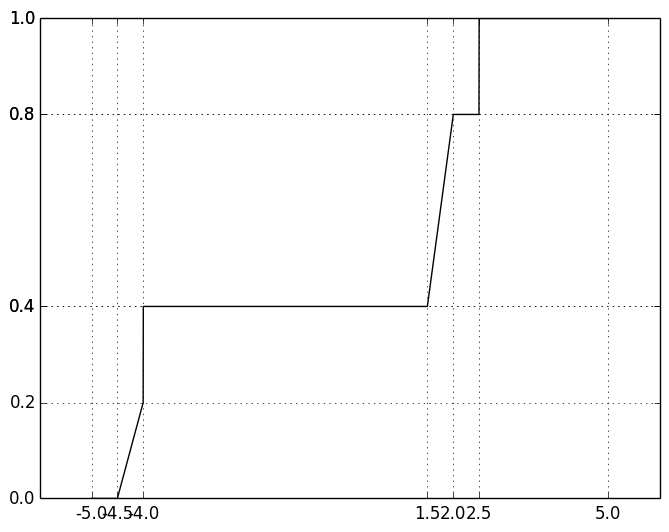
\includegraphics[width=0.8\linewidth]{/opt/webwork/courses/UCSD_CSE103/templates/setFinals/mixture_cdf_4.png}


{\pgmlSetup
Identify the component distributions:
\vskip\baselineskip
{\pgmlIndent\let\pgmlItem=\pgmlbulletItem
\pgmlItem{}Uniform component on the interval (\mbox{\parbox[t]{3.5ex}{\hrulefill}},\mbox{\parbox[t]{3ex}{\hrulefill}}). Its component weight is \mbox{\parbox[t]{3ex}{\hrulefill}}

\pgmlItem{}Uniform component on the interval (\mbox{\parbox[t]{3.5ex}{\hrulefill}},\mbox{\parbox[t]{3ex}{\hrulefill}}). Its component weight is \mbox{\parbox[t]{3ex}{\hrulefill}}

\pgmlItem{}Point mass on \mbox{\parbox[t]{3.5ex}{\hrulefill}}. Its component weight is \mbox{\parbox[t]{3ex}{\hrulefill}}

\pgmlItem{}Point mass on \mbox{\parbox[t]{3.5ex}{\hrulefill}}. Its component weight is \mbox{\parbox[t]{3ex}{\hrulefill}}

\par}%
\par}%
%%%%%%%%%%%%%%%%%%%%%%%%%%%%%%%%%%%%%%%%%%%%%%%%%%%%%%%%%%%%%%%%%%%%%%%%%%%%%%%%
% WeBWorK Online Homework Delivery System
% Copyright � 2000-2007 The WeBWorK Project, http://openwebwork.sf.net/
% $CVSHeader: webwork2/conf/snippets/hardcopyProblemDivider.tex,v 1.3 2004/06/24 21:10:50 dpvc Exp $
% 
% This program is free software; you can redistribute it and/or modify it under
% the terms of either: (a) the GNU General Public License as published by the
% Free Software Foundation; either version 2, or (at your option) any later
% version, or (b) the "Artistic License" which comes with this package.
% 
% This program is distributed in the hope that it will be useful, but WITHOUT
% ANY WARRANTY; without even the implied warranty of MERCHANTABILITY or FITNESS
% FOR A PARTICULAR PURPOSE.  See either the GNU General Public License or the
% Artistic License for more details.
%%%%%%%%%%%%%%%%%%%%%%%%%%%%%%%%%%%%%%%%%%%%%%%%%%%%%%%%%%%%%%%%%%%%%%%%%%%%%%%%

\medskip
\goodbreak
\hrule
\nobreak
\smallskip
{\bf 11.} (10 pts) \ifdim\lastskip=\pgmlMarker
  \let\pgmlPar=\relax
 \else
  \let\pgmlPar=\par
  \vadjust{\kern3pt}%
\fi

%%%%%%%%%%%%%%%%%%%%%%%%%%%%%%%%%%%%%%
%
%    definitions for PGML
%

\ifx\pgmlCount\undefined  % don not redefine if multiple files load PGML.pl
  \newcount\pgmlCount
  \newdimen\pgmlPercent
  \newdimen\pgmlPixels  \pgmlPixels=.5pt
\fi
\pgmlPercent=.01\hsize

\def\pgmlSetup{%
  \parskip=0pt \parindent=0pt
%  \ifdim\lastskip=\pgmlMarker\else\par\fi
  \pgmlPar
}%

\def\pgmlIndent{\par\advance\leftskip by 2em \advance\pgmlPercent by .02em \pgmlCount=0}%
\def\pgmlbulletItem{\par\indent\llap{$\bullet$ }\ignorespaces}%
\def\pgmlcircleItem{\par\indent\llap{$\circ$ }\ignorespaces}%
\def\pgmlsquareItem{\par\indent\llap{\vrule height 1ex width .75ex depth -.25ex\ }\ignorespaces}%
\def\pgmlnumericItem{\par\indent\advance\pgmlCount by 1 \llap{\the\pgmlCount. }\ignorespaces}%
\def\pgmlalphaItem{\par\indent{\advance\pgmlCount by `\a \llap{\char\pgmlCount. }}\advance\pgmlCount by 1\ignorespaces}%
\def\pgmlAlphaItem{\par\indent{\advance\pgmlCount by `\A \llap{\char\pgmlCount. }}\advance\pgmlCount by 1\ignorespaces}%
\def\pgmlromanItem{\par\indent\advance\pgmlCount by 1 \llap{\romannumeral\pgmlCount. }\ignorespaces}%
\def\pgmlRomanItem{\par\indent\advance\pgmlCount by 1 \llap{\uppercase\expandafter{\romannumeral\pgmlCount}. }\ignorespaces}%

\def\pgmlCenter{%
  \par \parfillskip=0pt
  \advance\leftskip by 0pt plus .5\hsize
  \advance\rightskip by 0pt plus .5\hsize
  \def\pgmlBreak{\break}%
}%
\def\pgmlRight{%
  \par \parfillskip=0pt
  \advance\leftskip by 0pt plus \hsize
  \def\pgmlBreak{\break}%
}%

\def\pgmlBreak{\\}%

\def\pgmlHeading#1{%
  \par\bfseries
  \ifcase#1 \or\huge \or\LARGE \or\large \or\normalsize \or\footnotesize \or\scriptsize \fi
}%

\def\pgmlRule#1#2{%
  \par\noindent
  \hbox{%
    \strut%
    \dimen1=\ht\strutbox%
    \advance\dimen1 by -#2%
    \divide\dimen1 by 2%
    \advance\dimen2 by -\dp\strutbox%
    \raise\dimen1\hbox{\vrule width #1 height #2 depth 0pt}%
  }%
  \par
}%

\def\pgmlIC#1{\futurelet\pgmlNext\pgmlCheckIC}%
\def\pgmlCheckIC{\ifx\pgmlNext\pgmlSpace \/\fi}%
{\def\getSpace#1{\global\let\pgmlSpace= }\getSpace{} }%

{\catcode`\ =12\global\let\pgmlSpaceChar= }%
{\obeylines\gdef\pgmlPreformatted{\par\small\ttfamily\hsize=10\hsize\obeyspaces\obeylines\let^^M=\pgmlNL\pgmlNL}}%
\def\pgmlNL{\par\bgroup\catcode`\ =12\pgmlTestSpace}%
\def\pgmlTestSpace{\futurelet\next\pgmlTestChar}%
\def\pgmlTestChar{\ifx\next\pgmlSpaceChar\ \pgmlTestNext\fi\egroup}%
\def\pgmlTestNext\fi\egroup#1{\fi\pgmlTestSpace}%

\def^^M{\ifmmode\else\space\fi\ignorespaces}%
%%%%%%%%%%%%%%%%%%%%%%%%%%%%%%%%%%%%%%
{\pgmlSetup
The {\bfseries{}Percentile} algorithm finds the $i$'th smallest element of an (unsorted) array of numbers. The {\bfseries{}Median} algorithm is the special case Percentile($S$,round($|S|/2))$.
\pgmlRule{100\pgmlPercent}{1\pgmlPixels}%
where we use $|S|$ to denote the length of the array $S$
\pgmlRule{100\pgmlPercent}{1\pgmlPixels}%
{\bfseries{}function} Percentile(S,i)
{\pgmlIndent\let\pgmlItem=\pgmlbulletItem
\pgmlItem{}Pick an element $v$ from $S$ at random
\pgmlItem{}Split $S$ into three pieces:\pgmlBreak
   - $S_L$, elements less than $v$\pgmlBreak
   - $S_v$, elements equal to $v$\pgmlBreak
   - $S_R$, elements greater than $v$ 

\pgmlItem{}If $i<|S_L|$  Return Percentile($S_L$,i)

\pgmlItem{}Else if $i<|S_L|+|S_v|$ return $v$

\pgmlItem{}Else Return Percentile($S_R$,i-{\ttfamily\char124}S{\itshape{}L{\ttfamily\char124}+{\ttfamily\char124}S}v{\ttfamily\char124})
\par}%
\vskip\baselineskip
\pgmlRule{100\pgmlPercent}{1\pgmlPixels}%
\vskip\baselineskip
In this problem, we find out some simple facts regarding the performance of the algorithm.
\vskip\baselineskip
A call to Percentile results either with the answer being found, or, in the more common case, a recursive call to Percentile with a shorter array.
\vskip\baselineskip
Clearly, the algorithm makes more progress the shorter the list with which the recursive call is made. We can't know whether the list that would be used is $S_L$ or $S_R$, we therefor want both to be short.
\vskip\baselineskip
{\pgmlIndent\let\pgmlItem=\pgmlbulletItem
\pgmlItem{}What is the probability of choosing v so that $|S_L|<\frac{3}{4} |S|$?  \mbox{\parbox[t]{3ex}{\hrulefill}}

\pgmlItem{}What is the probability of choosing v so that $|S_R|<\frac{3}{4} |S|$?  \mbox{\parbox[t]{3ex}{\hrulefill}}

\pgmlItem{}What is the probability of choosing v so that both $|S_R|<\frac{3}{4} |S|$
and $|S_L|<\frac{3}{4} |S|$?  \mbox{\parbox[t]{3ex}{\hrulefill}}
\vskip\baselineskip
\pgmlItem{}We call a split of the last type, where both $|S_R|<\frac{3}{4} |S|$
and $|S_L|<\frac{3}{4} |S|$, a {\bfseries{}good} split. What is the expected number of splits until we get a good split? \mbox{\parbox[t]{3.5ex}{\hrulefill}}
\vskip\baselineskip
\pgmlItem{}How many good splits do we need before the length of the list is reduced to one and the algorithm has to terminate? (Write your answer in terms of the length of the original list $|S|=n$) \mbox{\parbox[t]{4.5ex}{\hrulefill}}
\vskip\baselineskip
\pgmlItem{}Upper bound the expected number of splits (and recursive calls) before the algorithm terminates? \mbox{\parbox[t]{6.5ex}{\hrulefill}}

\par}%
\par}%
 \end{multicols}


\noindent {\tiny Generated by \copyright WeBWorK, http://webwork.maa.org, Mathematical Association of America}

 \begin{multicols}{2}
\columnwidth=\linewidth


%%%%%%%%%%%%%%%%%%%%%%%%%%%%%%%%%%%%%%%%%%%%%%%%%%%%%%%%%%%%%%%%%%%%%%%%%%%%%%%%
% WeBWorK Online Homework Delivery System
% Copyright � 2000-2007 The WeBWorK Project, http://openwebwork.sf.net/
% $CVSHeader: webwork2/conf/snippets/hardcopyPostamble.tex,v 1.2 2003/12/09 01:12:29 sh002i Exp $
% 
% This program is free software; you can redistribute it and/or modify it under
% the terms of either: (a) the GNU General Public License as published by the
% Free Software Foundation; either version 2, or (at your option) any later
% version, or (b) the "Artistic License" which comes with this package.
% 
% This program is distributed in the hope that it will be useful, but WITHOUT
% ANY WARRANTY; without even the implied warranty of MERCHANTABILITY or FITNESS
% FOR A PARTICULAR PURPOSE.  See either the GNU General Public License or the
% Artistic License for more details.
%%%%%%%%%%%%%%%%%%%%%%%%%%%%%%%%%%%%%%%%%%%%%%%%%%%%%%%%%%%%%%%%%%%%%%%%%%%%%%%%

\end{multicols}
\vfill
\end{document}
